%
%  kant.three
%
%  Created by Mark Eli Kalderon on 2007-08-05.
%  Copyright (c) 2007 Mark Eli Kalderon. All rights reserved.
%
%  Beamer

% Definitions and macros
\newcommand{\change}{\textcolor{blue}{\textbf{CHANGE SLIDE}}}
\newcommand\myauthor{Mark Eli Kalderon} 
\newcommand\mytitle{Introduction to Moral Philosophy}
\newcommand\mysubtitle{Kant}
\newcommand\myinstitution{University College London}
\newcommand\myurl{http://markelikalderon.com/teaching/}

% Packages specific to lecture notes
\mode<article>{
	\usepackage{palatino}
}

% Packages specific to beamer presentation
\mode<presentation>{
	\usetheme{Darmstadt}
	\setbeamercovered{transparent}
	\pgfdeclareimage[height=0.5cm]{university-logo}{../../graphics/logo_sml_blk}
	\logo{\pgfuseimage{university-logo}}
}

% Packages common to lecture notes and beamer presentation
\usepackage{pgf}
\usepackage{tikz}
\usepackage{hyperref}

\setjobnamebeamerversion{kant.three.beamer}

\title{\mytitle}
\subtitle{\mysubtitle} % (optional)

\author{\myauthor\\
\url{\myurl}}
\institute{\myinstitution}

% \date[Short Occasion] % (optional)
% {Date / Occasion}

\begin{document}

\frame{\maketitle}

\section{Review}\label{sec:review} % (fold)

\change\ In the first section, Kant seeks to answer the question, ``What is the supreme principle of morality?'', by appealing only to common rational moral cognition---the prereflective, practical knowledge of the rational standards that everyone implicitly uses in moral reasoning and judgment. Appealing only to such knowledge, Kant explicates the concept of the good will by considering the related concept of duty which leads Kant to characterize the supreme principle of morality in terms of the Formula of Universal Law. Kant's conclusion is conditional: If the supreme principle of morality exists, then its content is captured, at least in part, by the Formula of Universal Law.

In the second section, Kant reconsiders the question, ``What is the su\-preme principle of morality?''. Here, however, his arguments outstrip what is given by common rational moral cognition and have a more theoretical character. Instead of appealing only to prereflective, practical knowledge, Kant instead appeals to reflective, theoretical knowledge. \change

Another difference from the first section is that on the basis of such knowledge, Kant is able to give a richer characterization of the supreme principle of morality in terms of a system of three formulas, two of which have variant formulations. Again, Kant's conclusion is conditional: If the supreme principle of morality exists, then its content is captured by the system of three formulas. Kant claims that the three formulas reprsent the same principle and that they differ only in representing different aspects of the same principle. \change

A third difference is the argumentative strategy pursued. Instead of explicating the concept of the good will by considering duty, Kant, in the second section, derives the supreme principle of morality from the concept of a categorical imperative.

\emph{Hypothetical imperatives} presuppose the adoption of an end and prescribe an action as a means to achieving that end. The normative force of an hypothetical imperative is conditional on the adoption of the antecedent end: If a rational being has not adopted that end, then he is not required to perform the action prescribed as a means to that end.

In contrast, the normative force of a \emph{categorical imperative} is not conditional upon the adoption of any antecedent end: A rational being is required to perform the relevant action whatever ends he may in fact have adopted. \change

\begin{frame}<presentation>[label=slide1]
    \frametitle{The Strategy of Section Two}
        \begin{itemize}
            \item<1-> Whereas the argument of section one appeals to \alert{prereflective}, \alert{practical} knowledge, the argument of section two appeals to \alert{reflective}, \alert{theoretical} knowledge.
            \item<2-> Whereas the supreme principle of morality is characterized in section one in terms of the \alert{Formula of Universal Law}, section two characterizes the supreme principle of morality in terms of \alert{a system of three formulas}.
            \item<3-> Whereas the argument of section one proceeds by reflecting on the concept of the \alert{good will}, the argument of section two proceeds by reflecting on the concept of a \alert{categorical imperative}.
        \end{itemize}
\end{frame}

% section review (end)

\section{The Derivation of the First Formula}\label{sec:the_derivation} % (fold)

Today we will be talking about the derivation and application of the first formula. The first formula of the supreme principle of morality specifies the \emph{form} of the moral law (G 4:436) and has two variants:

\begin{enumerate}
	\item \emph{The Formula of Universal Law}: ``Act only in accordance with that maxim through which you can at the same time will that it become a universal law.'' (G 4:421; 4:402)
    \item \emph{The Formula of the Law of Nature}: ``Act as if the maxim of your action were to become by your will a universal law of nature.'' (G 4:421; 4:436)
\end{enumerate}

\change

\begin{frame}<presentation>[label=slide2]
    \frametitle{The Two Variants of the First Formula}
        \begin{columns}
            \begin{column}{3cm}
                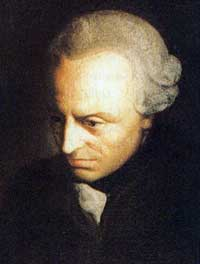
\includegraphics[height=4cm]{../../graphics/kant.jpg}
            \end{column}
            \begin{column}{7cm}
                \begin{itemize}
                	\item \alert{The Formula of Universal Law}: ``Act only in accordance with that maxim through which you can at the same time will that it become a universal law.'' (G 4:421; 4:402)
                    \item \alert{The Formula of the Law of Nature}: ``Act as if the maxim of your action were to become by your will a universal law of nature.'' (G 4:421; 4:436)
                \end{itemize}
            \end{column}
        \end{columns}
\end{frame}

Kant distinguishes two kinds of imperative:

\begin{enumerate}
  \item Hypothetical imperatives
  \item Categorical imperatives
\end{enumerate}

\emph{Hypothetical imperatives} presuppose the adoption of an end and prescribe an action as a means to achieving that end. The normative force of an hypothetical imperative is conditional on the adoption of the antecedent end: If a rational being has not adopted that end, then he is not required to perform the action prescribed as a means to that end.

In contrast, the normative force of a \emph{categorical imperative} is not conditional upon the adoption of any antecedent end: A rational being is required to perform the relevant action whatever ends he may in fact have adopted.

Two points of clarrification. First, Kant is not making any grammatical distinctions. Imperatives can be expressed by sentences in the indicative mood:

\begin{quote}
  Aiding those in the need is a good thing to do.
\end{quote}

Similarly, categorical imperatives, though unconditional, can be expressed by a conditional sentence:

\begin{quote}
  If you make a promise, keep it
\end{quote}

while hypothetical imperatives, though conditional, need not. Thus:

\begin{quote}
  Look out!
\end{quote}

can express the hypothetical imperative to pay attention to some immanent danger if you have adopted the end of avoiding bodily injury. Second, the claim that categorical imperatives are unconditional and so not dependent upon the adoption of some antecedent end is easily misunderstood. Kant is not claiming that a categorical imperative requires a person to act without an end. According to Kant, every action involves an end (Ms 6:384f). Rather, a categorical imperative is a requirement to adopt a particular end. \change

\begin{frame}<presentation>[label=slide3]
    \frametitle{Hypotehtical and Categorical Imperatives}
        \begin{columns}
            \begin{column}{3cm}
                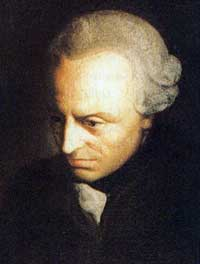
\includegraphics[height=4cm]{../../graphics/kant.jpg}
            \end{column}
            \begin{column}{7cm}
                \begin{itemize}
                    \item \alert{Hypothetical Imperatives} presuppose the adoption of an antecedent end and prescribe an action as the means to that end.
                    \item \alert{Categorical Imperatives} do not presuppose the adoption of an antecedent end: A rational being is required to perform the relevant action whatever ends he may in fact have adopted.
                \end{itemize}
            \end{column}
        \end{columns}
\end{frame}

Kant thinks that a characterization of the supreme principle of morality follows from the concept of the categorical imperative. The existence of such a principle does not follow from the concept of a categorical imperative. Given the overall argumentative structure of the Groundwork, the question of the existence of categorical imperatives is postponed until the third section. Rather, what follows from the concept of a categorical imperative, is merely that if there were categorical imperatives, they would have a certain characterization, that is, they would be represented by the two variations of the first formula. The characterization is formal in that it abstracts from the value that grounds the imperative and considers only the form of categorical requirements:

\begin{quote}
	When I think of a hypothetical imperative in general I do not know beforehand what it will contain; I do not know this until I am given the condition. But when I think of a categorical imperative I know at once what it contains. For, since the imperative contains, beyond the law, only the necessity that the maxim be in conformity with this law, while the law contains no condition to which it would be limited, nothing is left with which the maxim of action is to conform but the universality of a law as such; and this conformity alone is what the imperative properly represents as necessary. (G 4:420-421)
\end{quote}

A \emph{maxim} is a rule or policy governing action that a person adopts, at least implicitly, whenever they act. A categorical imperative requires a person to adopt maxims in conformity with with the law. The law is based on objective grounds, that is, grounds valid for every rational being (G 4:413). They are thus univerally valid rational requirements on action. Thus from the mere concept of a categorical imeprative Kant provisionally concludes that a categorical imperative requires that a person adopt maxims in conformity with the universality of law as such. \change

At this point, from the claim:

\begin{quote}
	Categorical imperatives require that a person adopts only maxims that conform to the universality of law as such.
\end{quote}

Kant concludes:

\begin{quote}
	There is, therefore, only a single categorical imperative and it is this: act only in accordance with that maxim through which you can at the same time will that it become a universal law. (G 4:421)
\end{quote}

This is essentially the same derivation of the Formula of Universal Law that Kant gave in the first section (G 4:402) and is therefore subject to the same difficulty. While the moral law may be valid for all rational beings, we so far have been given no reason to suppose that the law necessarily involves what a person could or could not will. Put another way, from the the fact that maxims should conform to universal law it does not follow that the will of a rational being has any role in determining the content of the law. Just as the Formula of Universal Law not follow from the concept of a categorical imperative neither does the other variant of the first formula, the Formula of the Law of Nature, and for precisely the same reason.

Kant is plausibly anticipating the idea of autonomy here for if rational beings are the authors of the moral law, then what rational beings could coherently will would be relevant to determining the content of that law. This undercores the way in which the three formulations of the supreme principle of morality should be read in light of the others. \change

\begin{frame}<presentation>[label=slide4]
    \frametitle{The Derivation}
        \begin{columns}
            \begin{column}{3cm}
                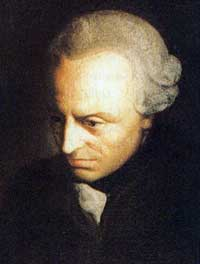
\includegraphics[height=4cm]{../../graphics/kant.jpg}
            \end{column}
            \begin{column}{7cm}
                \begin{itemize}
                    \item<1-> \alert{Categorical imperatives} require that a person adopts only maxims that conform to the universality of law as such.
                    \item<2-> From this Kant concludes: ``There is, therefore, only a single categorical imperative and it is this: \alert{act only in accordance with that maxim through which you can at the same time will that it become a universal law.}''
                \end{itemize}
            \end{column}
        \end{columns}
\end{frame}

% section the_derivation (end)

\section{The Formula of the Law of Nature}\label{sec:the_formula_of_the_law_of_nature} % (fold)

The Formula of Universal Law is abstract and so difficult to apply, but Kant thinks that it is easier and more intuitive to apply the Formula of the Law of Nature in determining the permissibility of a maxim. The Formula of Universal Law differs from the Formula of the Law of Nature in that the former involves willing a law whereas the latter involves willing a law of nature. A law is necessary in the sense that there are reasons that rational beings must conform to it. A law of nature, on the other hand, is necessary in a distinct sense. Specifically, it is causally impossible for rational beings to act contrary to a law of nature. Kant's idea is that we can gain an intutive understanding of which maxims we can will as a universal law by imagining a generalized form of the maxim as a law of nature conjoined to the actual laws of nature as we understand them and by asking whether we could coherently will that the resulting system of nature obtain. \change

\begin{frame}<presentation>[label=slide5]
    \frametitle{The Formula of the Law of Nature}
        \begin{columns}
            \begin{column}{6cm}
                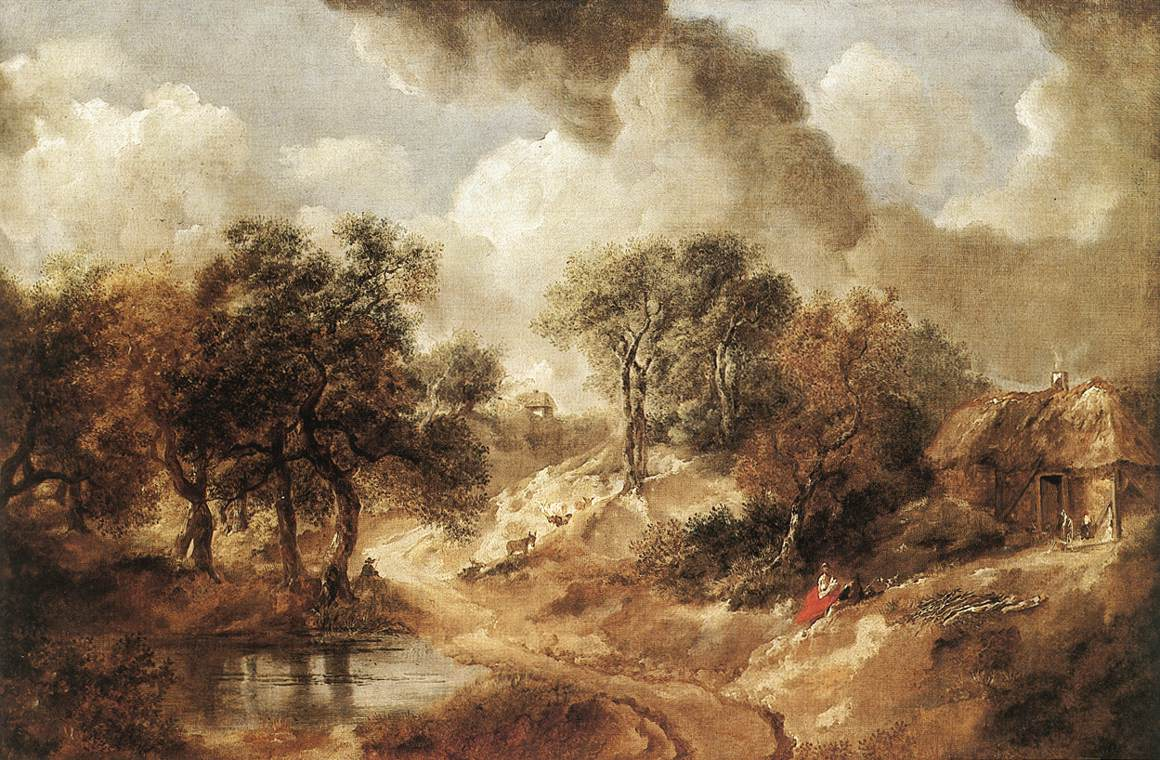
\includegraphics[height=4cm]{../../graphics/nature.jpg}
            \end{column}
            \begin{column}{4cm}
                Kant's idea is that we can gain an intuitive understanding of which maxims we can will as a universal law by imagining a generalized form of the maxim as a law of nature conjoined to the existing laws of nature as we understand them and by asking  whether we could coherently will that the resulting system of nature obtain.
            \end{column}
        \end{columns}
\end{frame}

The first step in applying the Formula of the Law of Nature is to specify the maxim to be tested:

\begin{quote}
	I am to perform action A in circumstances C in order to bring about end E.
\end{quote}

The second step is to generalize the maxim so that it applies to everyone:

\begin{quote}
	Everyone is to perform action A in circumstances C in order to bring about end E
\end{quote}
.
The third step is to transform the generalized maxim into a law of nature:

\begin{quote}
	It is a law of nature that everyone performs action A in circumstances C in order to bring about end E.
\end{quote}

The fourth step is to conjoin the hypothetical law of nature to the existing laws of nature and to work out the consequences of this in determining the new system of nature:

\begin{quote}
	Conjoin the hypothetical law of nature to the laws of nature as we understand them and work out what the system of nature would be once the effects of conjoining the novel law stabilize.
\end{quote}

The target maxim is permissible just in case one can coherently will the resulting system of nature. \change

\begin{frame}<presentation>[label=slide6]
    \frametitle{Four Steps}
        \begin{enumerate}
            \item The first step is to specify the maxim to be tested.
            \item The second step is to generalize the maxim.
            \item The third step is transform the generalized maxim into a law of nature.
            \item The fourth step is to conjoin the hypothetical law of nature to the existing laws of nature and to work out the consequences of this in determining the new system of nature.
        \end{enumerate}
        \alert{The target maxim is permissible just in case one can coherently will the resulting system of nature.}
\end{frame}

Kant distinguishes two tests for whether a person can coherently will the hypothetical system of nature:

\begin{enumerate}
	\item \emph{Contradiction in Conception}: The hypothetical system of nature cannot be conceived without self-contradiction.
    \item \emph{Contradiction in Volition}: The hypothetical system of nature cannot be willed without contradictory volition.
\end{enumerate}

As we will see, for Kant, this is a morally significant distinction. We can get a clearer understanding about these tests and the procedure involved in applying the Formula of the Law of Nature by working through Kant's four examples. \change

\begin{frame}<presentation>[label=slide7]
    \frametitle{Two Forms of Incoherence}
        \begin{columns}
            \begin{column}{3cm}
                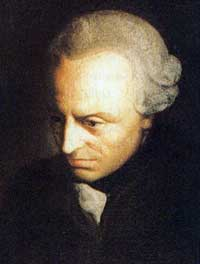
\includegraphics[height=4cm]{../../graphics/kant.jpg}
            \end{column}
            \begin{column}{7cm}
                \begin{itemize}
                    \item \alert{Contradiction in Conception}: The hypothetical system of nature cannot be conceived without self-contradiction.
                    \item \alert{Contradiction in Volition}: The hypothetical system of nature cannot be willed without contradictory volitions.
                \end{itemize}
            \end{column}
        \end{columns}
\end{frame}

In the first example, Kant argues that the following maxim fails to be permissible:

\begin{quote}
	\ldots from self-love I make it my principle to shorten my life when its longer duration threatens more troubles than it promises agreeableness. (G 4:422)
\end{quote}

Generalizing this maxim so that it applies to everyone, we get:

\begin{quote}
	From self-love everyone makes it their principle to shorten their life when its longer duration threatens more troubles than it promises agreeableness.
\end{quote}

Transforming this generalized maxim into a hypothetical law of nature we get:

\begin{quote}
	It is a law of nature that from self-love everyone makes it their principle to shorten their life when its longer duration threatens more troubles than it promises agreeableness.
\end{quote}

The next step is to determine whether we can, without self-contradiction, conjoin this hypothetical law of nature to the existing laws of nature as we understand them. Kant argues that we cannot and hence the maxim is impermissible:

\begin{quote}
	\ldots a nature whose law it would be to destroy life itself by means of the same feeling whose destination is to impel toward the furtherance of life would contradict itself and would therefore not subsist as nature; thus that maxim could not possibly be a law of nature and, accordingly, altogether opposes the supreme principle of all duty. (G 4:422)
\end{quote}

Kant's idea is that we cannot, without self-contradiction, conjoin the hypothetical law of nature to the existing laws of nature as we understand them given our teleological understanding of nature. Specifically, the following principle, according to Kant, is part of our understanding of nature:

\begin{quote}
	\emph{The Principle of Natural Teleology}: If $F$ is a feeling whose natural function is to produce effect $E$, then it would be self-contradictory to suppose that there could be a system of nature that includes a law that under circumstances $C$ $F$ produces the contrary of $E$.
\end{quote}

Since self-love has the natural function of furthering life, it is self-contradictory to suppose that there could be a system of nature that includes a law that under circumstances of more troubles than agreeableness self-love endeavors to shorten life. Since we cannot coherently suppose that there could be such a system of nature, we cannot coherently will that there should be such a system of nature, and hence the maxim of shortening life from self love when its longer duration threatens more troubles than agreeableness is impermissible.

Interestingly, Kant's argument here is controversial less for its deployment of the Formula of the Law of Nature and the contradiction in conception test than for its application of the principle of natural teleology. Specifically, after Darwin, it is controversial whether nature is in fact teleological in the way that Kant understands it to be. Even if it were, it would still be controversial whether self-love has the natural function that Kant assigns to it. \change

\begin{frame}<presentation>[label=slide8]
    \frametitle{Suicide}
        \begin{columns}
            \begin{column}{3cm}
                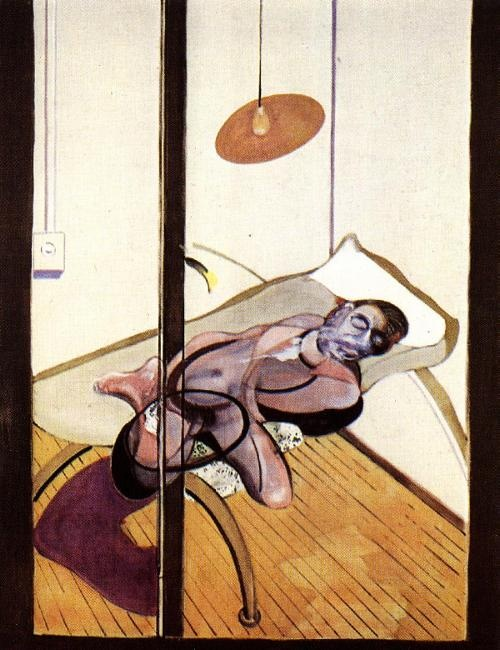
\includegraphics[height=4cm]{../../graphics/suicide.jpg}
            \end{column}
            \begin{column}{7cm}
                \begin{quote}
                    \ldots from self-love I make it my principle to shorten my life when its longer duration threatens more troubles than it promise agreeableness. (G4:422)
                \end{quote}
                \alert{The Principle of Natural Teleology}: If $F$ is a feeling whose natural function is to produce effect $E$, then it would be self-contradictory to suppose that there could be a system of nature that includes a law that under circumstances $C$ $F$ produces the contrary of $E$.
            \end{column}
        \end{columns}
\end{frame}

In the second example, Kant argues that the following maxim is impermissible:

\begin{quote}
	\ldots when I believe myself to be in need of money I shall borrow money and promise to repay it, even though I know that this will never happen. (G 4:422)
\end{quote}

Generalizing this maxim so that it applies to everyone, we get:

\begin{quote}
	When everyone believes themselves to be in need of money they will borrow money and promise to repay it, even though they know that this will never happen.
\end{quote}

Transforming this generalized maxim into a hypothetical law of nature we get:

\begin{quote}
	It is a law of nature that when everyone believes themselves to be in need of money they will borrow money and promise to repay it, even though they know that this will never happen.
\end{quote}

The next step is to determine whether we can, without self-contradiction, conjoin this hypothetical law of nature to the existing laws of nature as we understand them. Kant argues that we cannot and hence the maxim is impermissible:

\begin{quote}
	For, the universality of a law that everyone, when he believes himself to be in need, could promise whatever he pleases with the intention of not keeping it would make the promise and the end one might have in it itself impossible, since no one would believe what was promised but would laugh at all such expressions as vain pretenses. (G 4:422)
\end{quote}

Kant's idea is that we cannot, without self-contradiction, conjoin the hypothetical law of nature to the existing laws of nature as we understand them given the nature of promising. Specifically, the following principle governs the practice of promising:

\begin{quote}
	Promises are only possible if the promiser is justified in thinking that the promise will be believed.
\end{quote}

However, conjoining the hypothetical law with the existing laws of nature would bring it about that no promise is believed. Under such circumstances, no promise would be possible. Since we cannot coherently suppose that there could be such a system of nature, we cannot coherently will that there should be such a system of nature, and hence the maxim of borrowing money when in need of it and promising to repay it with no intention of doing so is impermissible. \change

\begin{frame}<presentation>[label=slide9]
    \frametitle{False Promises}
        \begin{columns}
            \begin{column}{4cm}
                
\includegraphics[height=4cm]{../../graphics/false_promises.jpg}
            \end{column}
            \begin{column}{6cm}
                \begin{quote}
                    \ldots when I believe myself to be in need of money I shall borrow money and promise to repay it, even though I know this will never happen. (G 4:422)
                \end{quote}
                \alert{A necessary condition on promising}: Promises are only possible if the promiser is justified in thinking that the promise will be believed.
            \end{column}
        \end{columns}
\end{frame}

While the previous examples deployed the contradiction in conception test, Kant's third and fourth examples deploy the contradiction in volition test. In the third example, Kant argues that the following maxim is impermissible:

\begin{quote}
	I will neglect the development of my natural talents and instead devote myself to idleness and pleasure.
\end{quote}

Generalizing this maxim so that it applies to everyone, we get:

\begin{quote}
	Everyone will neglect the development of their natural talents and instead devotes themselves to idleness and pleasure.
\end{quote}

Transforming this generalized maxim into a hypothetical law of nature we get:

\begin{quote}
	It is a law of nature that everyone neglects the development of their natural talents and instead devotes themselves to idleness and pleasure.
\end{quote}

However, Kant does not deny that we can, without self-contradiction, conjoin this hypothetical law of nature to the existing laws of nature as we understand them:

\begin{quote}
	\ldots nature could indeed always subsist with such a universal law, although (as with the South Sea Islanders) the human being should let his talents rust and be concerned with devoting his life merely to idleness, amusement, procreation---in a word, to enjoyment \ldots (G 4:423)
\end{quote}

While we can coherently conceive of the resulting system of nature, we cannot coherently will that such a system of nature obtain:

\begin{quote}
	For as a rational being he necessarily wills that all the capacities in him be developed, since they serve him and are given to him for all sorts of possible purposes. (G 4:423)
\end{quote}

This is an important and distinctively Kantian idea: that there are ends that every rational being must will. Kant, however, is less explicit about the specific rational principle from which he derives this result. (There are, however, plausible candidates available to Kant---rusting talents might be inconsistent with the counsels of prudence, for example.) \change

\begin{frame}<presentation>[label=slide10]
    \frametitle{Rusting Talents}
        \begin{columns}
            \begin{column}{5cm}
                
\includegraphics[height=4cm]{../../graphics/rusting_talents.jpg}
            \end{column}
            \begin{column}{5cm}
                I will neglect the development of my natural talents and instead devote myself to idleness and pleasure.
                \begin{quote}
                    For as a rational being he necessarily wills that all the capacities in him be developed, since they serve him and are given to him for all sorts of possible purposes. (G 4:423)
                \end{quote}
            \end{column}
        \end{columns}
\end{frame}

In the fourth example, Kant argues that the following maxim is impermissible:

\begin{quote}
	\ldots let each be as happy as heaven wills or as he can make himself; I shall take nothing from him nor even envy him; only I do not care to contribute to his welfare or to his assistance in need! (G 4:423)
\end{quote}

Generalizing this maxim so that it applies to everyone, we get:

\begin{quote}
	No one will harm anyone, but everyone will refuse to contribute to another's welfare or to provide assistance when in need.
\end{quote}

Transforming this generalized maxim into a hypothetical law of nature we get:

\begin{quote}
	It is a law of nature that no one harms anyone, but everyone refuses to contribute to another's welfare or to provide assistance when in need.
\end{quote}

However, Kant does not deny that we can, without self-contradiction, conjoin this hypothetical law of nature to the existing laws of nature as we understand them:

\begin{quote}
	Now, if such a way of thinking were to become a universal law the human race could admittedly very sell subsist, no doubt even better than when everyone prates about sympathy and beneveolence and even exerts himself to practice them occasionally, but on the other hand also cheats where he can, sells the rights of human beings or otherwise infringes upon them. (G 4:423)
\end{quote}

While we can coherently conceive of the resulting system of nature, we cannot coherently will that such a system of nature obtain:

\begin{quote}
	For, a will that decided this would conflict with itself, since many cases could occur in which one would need the love and sympathy of others in which, by such a law of nature arisen from his own will, he would rob himself of all hope of the assistance he wishes for himself. (G 4:423)
\end{quote}

\change

\begin{frame}<presentation>[label=slide11]
    \frametitle{Refusing Aid}
        \begin{columns}
            \begin{column}{3cm}
                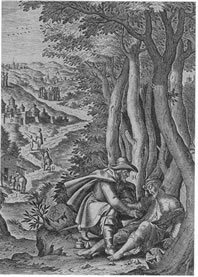
\includegraphics[height=5cm]{../../graphics/samaritan.jpg}
            \end{column}
            \begin{column}{7cm}
                \begin{quote}
                    \ldots let each be as happy as heaven wills or as he can make himself; I shall take nothing from him nor even envy him; only I do not care to contribute to his welfare or to his assistance in need! (G 4:423)\\
                    For, a will that decided this would conflict with itself, since many cases could occur in which one would need the love and sympathy of others in which, by such a law of nature arisen from his own will, he would rob himself of all hope of the assistance he wishes for himself. (G 4:423) 
                \end{quote}
            \end{column}
        \end{columns}
\end{frame}

How are we to understand the contradiction in volition?

In \emph{Utilitarianism}, Mill suggests that the contradiction in volition test should be understood as follows:

\begin{quote}
	To give any meaning to Kant's principle, the sense put upon it must be that we ought to shape our conduct by a rule which all rational beings might adopt with benefit to their collective interest.
\end{quote}

Unfortunately, the sense Mill puts upon Kant's principle could not be sense that Kant intends. Recall that Kant thinks that the system of nature in which no one harms anyone but everyone refuses aid is better than the existing system of nature, but the corresponding maxim is impermissible nonetheless. So the contradiction in volition could not be grounded in an appeal to utility as Mill evidently believed. \change

\begin{frame}<presentation>[label=slide12]
    \frametitle{Mill's Interpretation}
        \begin{columns}
            \begin{column}{3cm}
                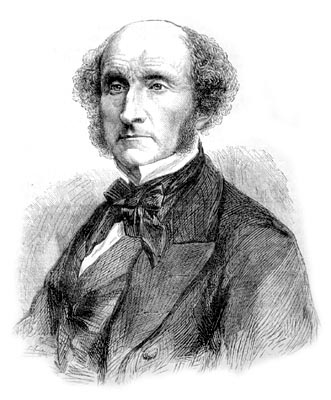
\includegraphics[height=4cm]{../../graphics/mill.jpg}
            \end{column}
            \begin{column}{7cm}
                \begin{quote}
                    To give any meaning to Kant's principle, the sense put upon it must be that we ought to shape our conduct by a rule which all rational beings might adopt \alert{with benefit to their collective interest}.
                \end{quote}
            \end{column}
        \end{columns}
\end{frame}

While Mill did not intend his interpretation of the contradiction in volition test as a criticism of Kant, Schopenhauer's interpretation of the test is so intended. According to Schopenhauer, Kant's application of the contradiction in volition test in the fourth example makes what would be, by Kant's lights, an illicit appeal to self-interest. After all, Kant does make a claim about what a person must will on the grounds of self-interest, i.e., that a person might require the aid of others and hence cannot rationally will that a system of nature obtain in which they are deprived of that aid. While Kant's argument does employ a premise about rational self-interest, Kant's conclusion is not grounded in an illicit appeal to self-interest. Kant is making a hypothetical claim about what would be in a person's self-interest if the maxim were a law of nature. No claim is being made about what is in fact in their interest given the existing laws of nature. So the duty to give aid is not grounded in what is in fact in a person's self-interest in the way that Schopenhauer suggests. \change

\begin{frame}<presentation>[label=slide13]
    \frametitle{Schopenhauer's Criticism}
        \begin{columns}
            \begin{column}{3cm}
                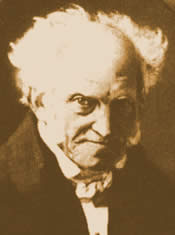
\includegraphics[height=4cm]{../../graphics/schopenhauer.jpg}
            \end{column}
            \begin{column}{7cm}
                Kant makes an illicit claim about what a person must will on the grounds of self-interest, i.e., that a person might require the aid of others and hence cannot rationally will that a system of nature obtain in which they are deprived of that aid. 
            \end{column}
        \end{columns}
\end{frame}

Kant's four examples are supposed to be exemplars of a fourfold division of duties. Specifically, Kant posits a pair of overlapping distinctions:

\begin{enumerate}
	\item Duties are distinguished with respect to their objects: There are duties to oneself and duties to other human beings.
    \item Duties are distinguished with respect to whether they admit of exception in favor of inclination There are imperfect duties that do not and perfect duties that do.
\end{enumerate}

This division of duties anticipates the more complex table of duties that Kant presents in The Metaphysics of Morals.

The division of duties into perfect and imperfect is suppposed to correspond to the two universalizability tests:

\begin{description}
	\item [ The Correspondence Thesis ] Maxims that violate perfect duties violate the contradiction in conception test; maxims that violate imperfect duties violate the contradiction in volition test.
\end{description}

Perfect duties admit of no exception in favor of inclination whereas imperfect duties do. How are we to understand this? In \emph{The Metaphysics of Morals}, Kant explains further. \emph{Perfect duties} are requirements on actions and any violation of a perfect duty is an instance of wrongdoing and hence blameworthy. \emph{Imperfect duties} are requirements on the adoption of ends though there is latitude in the fulfillment of these ends since a person has a variety of ends and these must be rationally ordered. (This is the sense in which they admit of exception in favor of inclination.) Specific actions taken toward the fulfillment of required ends is meritorious, whereas the failure to act toward the fulfillment of the required end merely lacks merit and is not an instance of wrongdoing and hence not blameworthy.

How plausible is the correspondence thesis? One difficulty is the existence of maxims that can be conceived without contradiction as a universal law of nature but where acting on that maxim violates a perfect duty. Consider the following maxim:

\begin{quote}
	I will kill another human being when it is a safe and effective way of furthering my self-interest.
\end{quote}

Generalizing this maxim we get:

\begin{quote}
	Everyone will kill another human being when it is a safe and effective way of furthering their self-interest.
\end{quote}

Transforming this generalized maxim into a law of nature we get:

\begin{quote}
	It is a law of nature that everyone will kill another human being when it is a safe and effective way of furthering their self-interest.
\end{quote}

While we may be unable to will the resulting system of nature (the system of nature that results from conjoining the hypothetical law of nature with the existing laws of nature), it is at least arguable that it can be conceived without contradiction. But to act on this maxim would be to violate a duty of justice and duties of justice are perfect duties if any are. \change

\begin{frame}<presentation>[label=slide14]
    \frametitle{The Table of Duties}
        \begin{tabular}{lll}
            \hline
            & \alert{Duties to Oneself} & \alert{Duties to Others}\\
            \hline
            \alert{Perfect Duties} & Suicide & False Promises\\
            \hline
            \alert{Imperfect Duties} & Rusting Talents & Refusing Aid\\
            \hline
        \end{tabular}
        
        \begin{block}{The Correspondence Thesis}
        	Maxims that violate perfect duties violate the contradiction in conception test; maxims that violate imperfect duties violate the contradiction in volition test.
        \end{block}
        
\end{frame}

% section the_formula_of_the_law_of_nature (end)

\section*{Next Time}\label{sec:next_time} % (fold)

% TODO: Add text and slide

% section next_time (end)
\end{document}
